\documentclass[tikz,border=10pt]{standalone}
\begin{document}
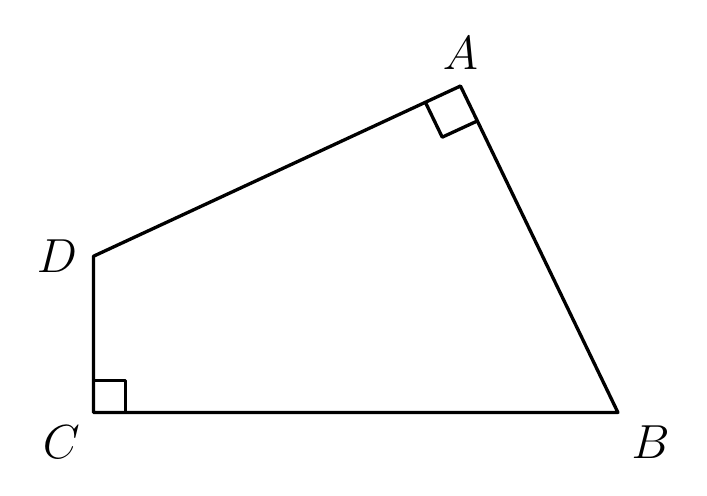
\begin{tikzpicture}[line join=round, line width=1.2pt]
% Vertices in cm: x=(px-227.75)*0.021108, y=(163.8-py)*0.021108
\coordinate (A) at (1.331,2.073);
\coordinate (B) at (3.330,-2.073);
\coordinate (C) at (-3.330,-2.073);
\coordinate (D) at (-3.330,-0.089);

% Quadrilateral ABCD (solid)
\draw (A) -- (B) -- (C) -- (D) -- cycle;

% Right angle at C (between CB and CD), one square mark
\draw (-2.924,-2.073) -- (-2.924,-1.667) -- (-3.330,-1.667);

% Right angle at A (between AB and AD), one square mark
\draw (0.885,1.866) -- (1.099,1.423) -- (1.545,1.629);

% Labels outside the figure
\node[above=2pt, font=\fontsize{17}{20.4}\selectfont] at (A) {$A$};
\node[below right=1pt, font=\fontsize{17}{20.4}\selectfont] at (B) {$B$};
\node[below left=1pt, font=\fontsize{17}{20.4}\selectfont] at (C) {$C$};
\node[left=2pt, font=\fontsize{17}{20.4}\selectfont] at (D) {$D$};
\end{tikzpicture}
\end{document}